\ffigbox[\FBwidth]{%
\caption{\centering Un graphe complet avec solution à \(P_1\)}\label{fig:dm1_ex02_f3}
}{
    \fbox{
        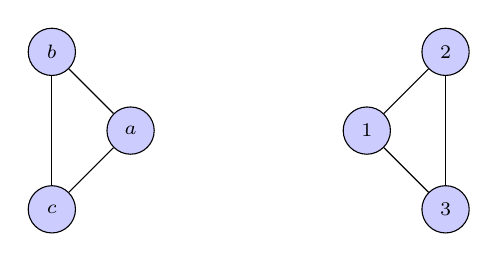
\begin{tikzpicture}[scale=1, main node/.style={circle, draw, fill=blue!20, inner sep=1pt, font=\scriptsize, minimum size=6mm, text=black}]
            % les sommets initiaux
            \node[main node] (a) at (0,0) {\(a\)};
            \node[main node] (b) at (-1,1) {\(b\)};
            \node[main node] (c) at (-1,-1) {\(c\)};
            
            \node[main node] (1) at (3,0) {\(1\)};
            \node[main node] (2) at (4,1) {\(2\)};
            \node[main node] (3) at (4,-1) {\(3\)};

            % les arcs avec capacités
            \draw (a) to (b);
            \draw (a) to (c);
            \draw (b) to (c);
            
            \draw (1) to (2);
            \draw (1) to (3);
            \draw (2) to (3);

        \end{tikzpicture}
    }
}